% https://www.zhihu.com/question/1955690045978699399/answer/2012283763393062517
\documentclass[tikz,border=5pt]{standalone}
\usetikzlibrary{arrows.meta,fit}
\usepackage{fourier}
\begin{document}

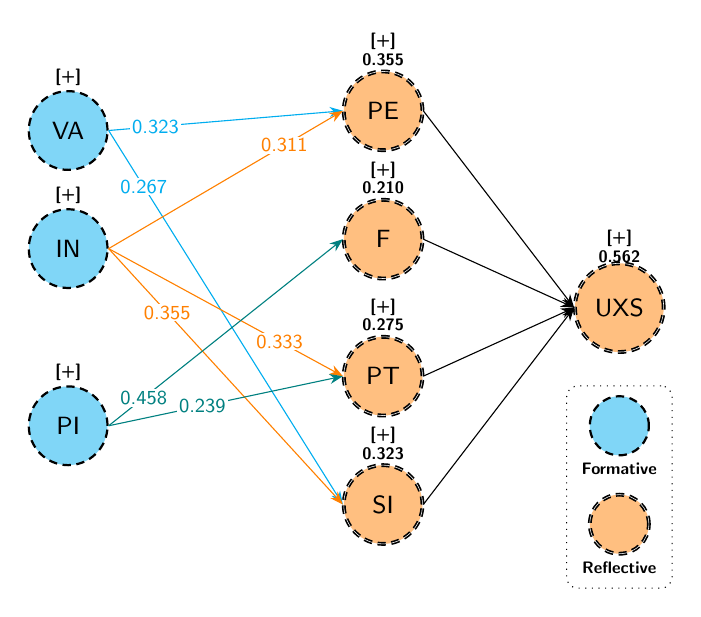
\begin{tikzpicture}[
    font=\sffamily\small,>=Stealth,
    base/.style={inner sep=5pt,circle,draw,densely dashed,minimum size=1cm},
    A/.style={base,fill=cyan!50,thick},
    B/.style={base,fill=orange!50,semithick,double,double distance=.2pt},
    edgenode/.style={rectangle,fill=white,inner sep=1pt,scale=.8},
    labelnode/.style={above=.5cm,anchor=south,align=center,scale=.6,font=\sffamily\bfseries},
    ]
    \node[A] (A1) at (-4,2.25) {VA};
    \node[A] (A2) at (-4,.75) {IN};
    \node[A] (A3) at (-4,-1.5) {PI};
    \node[B] (B1) at (0,2.5) {PE};
    \node[B] (B2) at (0,.87) {F};
    \node[B] (B3) at (0,-.87) {PT};
    \node[B] (B4) at (0,-2.5) {SI};
    \node[B] (C) at (3,0) {UXS};
    \path 
        (A1) node[labelnode] {[+]}
        (A2) node[labelnode] {[+]}
        (A3) node[labelnode] {[+]}
        (B1) node[labelnode] {[+]\\0.355}
        (B2) node[labelnode] {[+]\\0.210}
        (B3) node[labelnode] {[+]\\0.275}
        (B4) node[labelnode] {[+]\\0.323}
        (C) node[labelnode] {[+]\\0.562}
    ;
    \path (A1.east) 
        edge[->,cyan] node[edgenode,pos=.2,text=cyan] {0.323} (B1.west)
        edge[->,cyan] node[edgenode,pos=.15,text=cyan] {0.267} (B4.west)
        ;
    \path (A2.east) 
        edge[->,orange] node[edgenode,pos=.75,text=orange] {0.311} (B1.west)
        edge[->,orange] node[edgenode,pos=.73,text=orange] {0.333} (B3.west)
        edge[->,orange] node[edgenode,pos=.25,text=orange] {0.355} (B4.west)
        ;
    \path (A3.east) 
        edge[->,teal] node[edgenode,pos=.15,text=teal] {0.458} (B2.west)
        edge[->,teal] node[edgenode,pos=.4,text=teal] {0.239} (B3.west)
        ;
    \path (C.west)
        edge[<-] (B1.east)
        edge[<-] (B2.east)
        edge[<-] (B3.east)
        edge[<-] (B4.east) ;

    \path 
        (3,-1.5) node[A,minimum size=.75cm] (s1) {} 
                node[labelnode,below=1.5cm] (t1) {Formative} 
        (3,-2.75) node[B,minimum size=.75cm] (s2) {} 
                node[labelnode,below=1.5cm] (t2) {Reflective} 
        ;
    \node[fit=(s1)(s2)(t1)(t2),draw,dotted,rounded corners,rectangle] {};
\end{tikzpicture}

\end{document}